%%%%%%%%%%%%%%%%%%%%%%%%%%%%%%%%%%%%%%%%%%%%%%%%%%%%%%%%%%%%%%%%%%%%%%
% PACKAGES AND OTHER DOCUMENT CONFIGURATIONS
%%%%%%%%%%%%%%%%%%%%%%%%%%%%%%%%%%%%%%%%%%%%%%%%%%%%%%%%%%%%%%%%%%%%%%
\documentclass[final]{beamer}
\usepackage[scale=1]{beamerposter}
%%%%%%%%%%%%%%%%%%%%%%%%%%%%%%%%%%%%%%%%%%%%%%%%%%%%%%%%%%%%%%%%%%%%%%
% Define the column widths and overall poster size
%
% [original]
% To set effective sepwid, onecolwid and twocolwid values, first
% choose how many columns you want and how much separation you want
% between columns In this template, the separation width chosen is
% 0.024 of the paper width and a 4-column layout onecolwid should
% therefore be (1-(# of columns+1)*sepwid)/# of columns
% e.g. (1-(4+1)*0.024)/4 = 0.22 Set twocolwid to be
% (2*onecolwid)+sepwid = 0.464 Set threecolwid to be
% (3*onecolwid)+2*sepwid = 0.708
%
% [tk mod]
% sepwid = same as before
% tithewidth = (1-(# of col+1)*sepwid)/10 (# of col = 3)
%
% e.g. if three columns with width ratio 3:4:3 are desired use
% 3\tithewid, 4\tithewid, 3\tithewid.

\newlength{\sepwid}
\newlength{\onecolwid}
\newlength{\twocolwid}
\newlength{\threecolwid}
\newlength{\tithewid}
%% Arch E
\setlength{\paperwidth}{48in}
\setlength{\paperheight}{36in}
%% Arch E1
% \setlength{\paperwidth}{42in}
% \setlength{\paperheight}{30in}
% \setlength{\textwidth}{41.5in}
% \setlength{\textheight}{29.5in}
%% A0
% \setlength{\paperwidth}{46.8in}
% \setlength{\paperheight}{33.1in}
% \setlength{\sepwid}{0.024\paperwidth} % Separation width (white
% space) between columns

\setlength{\sepwid}{0.024\paperwidth} % Separation width (white space) between columns
\setlength{\tithewid}{0.0904\paperwidth}
% \setlength{\onecolwid}{0.22\paperwidth} % Width of one column
% \setlength{\twocolwid}{0.464\paperwidth} % Width of two columns
% \setlength{\threecolwid}{0.708\paperwidth} % Width of three columns
\setlength{\topmargin}{-0.5in} % Reduce the top margin size

%%%%%%%%%%%%%%%%%%%%%%%%%%%%%%%%%%%%%%%%%%%%%%%%%%%%%%%%%%%%%%%%%%%%%%
\usetheme{confposter}

\setbeamercolor{block title}{fg=ngreen,bg=white}
% \setbeamercolor{block title}{fg=nred,bg=white}
\setbeamercolor{block body}{fg=black,bg=white}
\setbeamercolor{block alerted title}{fg=white,bg=dblue!70}
\setbeamercolor{block alerted body}{fg=black,bg=dblue!10}
% Many more colors are available for use in beamerthemeconfposter.sty

%%%%%%%%%%%%%%%%%%%%%%%%%%%%%%%%%%%%%%%%%%%%%%%%%%%%%%%%%%%%%%%%%%%%%%

\addtobeamertemplate{block end}{}{\vspace*{2ex}} % White space under blocks
\addtobeamertemplate{block alerted end}{}{\vspace*{2ex}} % White space under highlighted (alert) blocks

\setlength{\belowcaptionskip}{2ex} % White space under figures
\setlength{\belowdisplayshortskip}{2ex} % White space under equations

\usepackage{graphicx}
\usepackage{booktabs}
\graphicspath{ {./figures/} }
\usepackage{multicol}

%%%% Custom macros

%% Greek letters
\newcommand{\al}{\alpha}
\newcommand{\be}{\beta}
\newcommand{\de}{\delta}
\newcommand{\e}{\epsilon}
\newcommand{\eps}{\varepsilon}
\newcommand{\g}{\gamma}
\newcommand{\ka}{\kappa}
\newcommand{\la}{\lambda}
\newcommand{\om}{\omega}
\newcommand{\Om}{\Omega}
\newcommand{\sig}{\sigma}
\let\oldth\th %% \th is used for "thorn"
\renewcommand{\th}{\theta}


%% Blackboard
\newcommand{\NN}{\mathbb{N}}
\newcommand{\ZZ}{\mathbb{Z}}
\newcommand{\QQ}{\mathbb{Q}}
\newcommand{\RR}{\mathbb{R}}
\newcommand{\CC}{\mathbb{C}}
\newcommand{\TT}{\mathbb{T}}
\newcommand{\DD}{\mathbb{D}}
\newcommand{\HH}{\mathbb{H}}
\newcommand{\UU}{\mathbb{U}}
\newcommand{\1}{\mathbbm{1}}

%% Caligraphic
\newcommand{\cA}{\mathcal{A}}
\newcommand{\cB}{\mathcal{B}}
\newcommand{\cC}{\mathcal{C}}
\newcommand{\cD}{\mathcal{D}}
\newcommand{\cE}{\mathcal{E}}
\newcommand{\cF}{\mathcal{F}}
\newcommand{\cG}{\mathcal{G}}
\newcommand{\cH}{\mathcal{H}}
\newcommand{\cI}{\mathcal{I}}
\newcommand{\cJ}{\mathcal{J}}
\newcommand{\cK}{\mathcal{K}}
\newcommand{\cL}{\mathcal{L}}
\newcommand{\cM}{\mathcal{M}}
\newcommand{\cN}{\mathcal{N}}
\newcommand{\cO}{\mathcal{O}}
\newcommand{\cP}{\mathcal{P}}
\newcommand{\cQ}{\mathcal{Q}}
\newcommand{\cR}{\mathcal{R}}
\newcommand{\cS}{\mathcal{S}}
\newcommand{\cT}{\mathcal{T}}
\newcommand{\cU}{\mathcal{U}}
\newcommand{\cV}{\mathcal{V}}
\newcommand{\cW}{\mathcal{W}}


%% Roman, italic, boldface
\newcommand{\bA}{\mathbf{A}}
\newcommand{\bB}{\mathbf{B}}
\newcommand{\bC}{\mathbf{C}}
\newcommand{\bD}{\mathbf{D}}
\newcommand{\bE}{\mathbf{E}}
\newcommand{\bI}{\mathbf{I}}
\newcommand{\bK}{\mathbf{K}}
\newcommand{\bL}{\mathbf{L}}
\newcommand{\bM}{\mathbf{M}}
\newcommand{\bN}{\mathbf{N}}
\newcommand{\bP}{\mathbf{P}}
\newcommand{\bS}{\mathbf{S}}
\newcommand{\bT}{\mathbf{T}}
\newcommand{\ba}{\mathbf{a}}
\newcommand{\bc}{\mathbf{c}}
\newcommand{\bd}{\mathbf{d}}
\newcommand{\bh}{\mathbf{h}}
\newcommand{\br}{\mathbf{r}}


%% Editorial
\renewcommand{\thefootnote}{(\arabic{footnote})}
% \setlength\parindent{0pt} % Removes all indentation from paragraphs


%% Delimiters, accents, bars, etc
\newcommand{\abs}[1]{\left|#1\right|}
\newcommand{\ceil}[1]{\left\lceil#1\right\rceil}
\newcommand{\floor}[1]{\left\lfloor#1\right\rfloor}
\newcommand{\conj}[1]{\overline{#1}}
\newcommand{\norm}[1]{\left\|#1\right\|}
\newcommand{\Norm}[2]{\left\|#1\right\|_{#2}}
\newcommand{\avg}[1]{\langle#1\rangle}


%% Mathematical functions and operators
\DeclareMathOperator{\re}{Re}
\DeclareMathOperator{\im}{Im}
\DeclareMathOperator{\sgn}{sgn}
\DeclareMathOperator{\erf}{erf}
\DeclareMathOperator{\erfc}{erfc}
\DeclareMathOperator{\ii}{i}
\DeclareMathOperator{\dd}{\,d}
\DeclareMathOperator{\eu}{e}
\newcommand{\del}{\partial}
\newcommand{\tri}{\triangle}
\newcommand{\grad}{\nabla}
\newcommand{\dvg}{\nabla\cdot}
\newcommand{\curl}{\nabla\times}
% \newcommand{\p}{'}
% \newcommand{\pp}{''}
% \newcommand{\ppp}{'''}


%% Principal value integral
\def\Xint#1{\mathchoice
   {\XXint\displaystyle\textstyle{#1}}%
   {\XXint\textstyle\scriptstyle{#1}}%
   {\XXint\scriptstyle\scriptscriptstyle{#1}}%
   {\XXint\scriptscriptstyle\scriptscriptstyle{#1}}%
   \!\int}
\def\XXint#1#2#3{{\setbox0=\hbox{$#1{#2#3}{\int}$}
     \vcenter{\hbox{$#2#3$}}\kern-.5\wd0}}
\def\ddashint{\Xint=}
\def\pvint{\Xint-}


%% Frequently used, projected spaces
\newcommand{\pl}[1]{#1_{\mathsmaller{\mathsmaller{<}}}} % proj. less than
\newcommand{\pg}[1]{#1_{\mathsmaller{\mathsmaller{>}}}} % proj. greater than
\newcommand{\hl}{\pl{\bh}} % h_<
\newcommand{\hg}{\pg{\bh}} % h_>
\newcommand{\gl}{\pl{g}} % g_<
\newcommand{\gG}{\pg{g}} % g_>, \gg is already taken
\newcommand{\El}{\pl{\bE}} % E_< (sequence)
\newcommand{\Eg}{\pg{\bE}} % E_> (sequence)
\newcommand{\eg}{\pg{E}} % E_> (function)
\newcommand{\rl}{\pl{\br}} % r_<
\newcommand{\rg}{\pg{\br}} % r_>
\newcommand{\Linf}{\mathrm{L}^{\infty}} % L^{\infty}
\newcommand{\Ltwo}{\mathrm{L}^2} % L^2


%% Frequently used, subscripted functions
\newcommand{\gone}{g_{1}}
\newcommand{\gtwo}{g_{2}}
\newcommand{\Eone}{E_{1}}
\newcommand{\Etwo}{E_{2}}
\newcommand{\eone}{E^{(1)}}
\newcommand{\etwo}{E^{(2)}}
\newcommand{\euone}{E_{u}^{(1)}}
\newcommand{\eutwo}{E_{u}^{(2)}}
\newcommand{\uone}{u^{(1)}}
\newcommand{\utwo}{u^{(2)}}
\newcommand{\Ez}{E^{(0)}}
\newcommand{\uz}{u^{(0)}}


%% Tilde-ed operators
\newcommand{\tcA}{\widetilde{\cA}}
\newcommand{\tF}{\widetilde{F}}
\newcommand{\tcK}{\widetilde{\cK}}
\newcommand{\tL}{\widetilde{L}}
\newcommand{\tcL}{\widetilde{\cL}}
\newcommand{\tM}{\widetilde{M}}
\newcommand{\tcM}{\widetilde{\cM}}
\newcommand{\tR}{\widetilde{R}}
\newcommand{\tcR}{\widetilde{\cR}}


%% Some shortcuts
\newcommand{\vu}{\vec{u}}
\newcommand{\vom}{\vec{\om}}
\newcommand{\dn}{\del_{\nu}}
\newcommand{\du}{\del_{u}}


%% Tweak some Greek letters
\newcommand{\bchi}{\mbox{\raisebox{.4ex}{\begin{large}$\chi$\end{large}}}}
\newcommand{\Chi}{\mbox{\Large$\chi$}} % nicer looking Chi
\newcommand{\bzeta}{\boldsymbol{\zeta}} % Riemann zeta function


%% Principal value integral
\def\Xint#1{\mathchoice
   {\XXint\displaystyle\textstyle{#1}}%
   {\XXint\textstyle\scriptstyle{#1}}%
   {\XXint\scriptstyle\scriptscriptstyle{#1}}%
   {\XXint\scriptscriptstyle\scriptscriptstyle{#1}}%
   \!\int}
\def\XXint#1#2#3{{\setbox0=\hbox{$#1{#2#3}{\int}$}
     \vcenter{\hbox{$#2#3$}}\kern-.5\wd0}}
\def\ddashint{\Xint=}
\def\pvint{\Xint-}


%% Arc over symbols
% reference: https://tex.stackexchange.com/questions/96680/a-better-notation-to-denote-arcs-for-an-american-high-school-textbook
\makeatletter
\DeclareFontFamily{U}{tipa}{}
\DeclareFontShape{U}{tipa}{m}{n}{<->tipa10}{}
\newcommand{\arc@char}{{\usefont{U}{tipa}{m}{n}\symbol{62}}}%
\newcommand{\arc}[1]{\mathpalette\arc@arc{#1}}
\newcommand{\arc@arc}[2]{%
  \sbox0{$\m@th#1#2$}%
  \vbox{
    \hbox{\resizebox{\wd0}{\height}{\arc@char}}
    \nointerlineskip
    \box0
  }%
}

\newsavebox{\astrutbox}
\sbox{\astrutbox}{\rule[-5pt]{0pt}{20pt}}
\newcommand{\astrut}{\usebox{\astrutbox}}
\newcommand{\rls}{\raisebox{2pt}{\tikz{\draw[red,solid,line width=0.9pt](0,0) -- (5mm,0);}}}
\newcommand{\rld}{\raisebox{2pt}{\tikz{\draw[red,dashed,line width=1.0pt](0,0) -- (5mm,0);}}}
\newcommand{\bls}{\raisebox{2pt}{\tikz{\draw[blue,solid,line width=0.9pt](0,0) -- (5mm,0);}}}
\newcommand{\bld}{\raisebox{2pt}{\tikz{\draw[blue,dashed,line width=1.0pt](0,0) -- (5mm,0);}}}
\newcommand{\gls}{\raisebox{2pt}{\tikz{\draw[green,solid,line width=0.9pt](0,0) -- (5mm,0);}}}
\newcommand{\gld}{\raisebox{2pt}{\tikz{\draw[green,dashed,line width=1.0pt](0,0) -- (5mm,0);}}}
\newcommand{\mls}{\raisebox{2pt}{\tikz{\draw[magenta,solid,line width=0.9pt](0,0) -- (5mm,0);}}}
\newcommand{\mld}{\raisebox{2pt}{\tikz{\draw[magenta,dashed,line width=1.0pt](0,0) -- (5mm,0);}}}
\newcommand{\cls}{\raisebox{2pt}{\tikz{\draw[cyan,solid,line width=0.9pt](0,0) -- (5mm,0);}}}
\newcommand{\cld}{\raisebox{2pt}{\tikz{\draw[cyan,dashed,line width=1.0pt](0,0) -- (5mm,0);}}}

\newcommand{\ds}{\displaystyle}

%% Defining theorem environment
\theoremstyle{definition}
\newtheorem{defn}{Definition}
\newtheorem{notn}[defn]{Notation}
\newtheorem{rmk}[defn]{Remark}
\newtheorem{cor}[defn]{Corollary}
\newtheorem{lem}[defn]{Lemma}
\newtheorem{thm}[defn]{Theorem}
\newtheorem{cons}[defn]{Consequence}
\newtheorem{conv}[defn]{Convention}
\newtheorem{prob}[defn]{Problem}
\newtheorem{form}[defn]{Formulation}
\newtheorem{claim}[defn]{Claim}



%%%%%%%%%%%%%%%%%%%%%%%%%%%%%%%%%%%%%%%%%%%%%%%%%%%%%%%%%%%%%%%%%%%%%%
% TITLE SECTION
%%%%%%%%%%%%%%%%%%%%%%%%%%%%%%%%%%%%%%%%%%%%%%%%%%%%%%%%%%%%%%%%%%%%%%
\title{Quasi-Solution Approach to a 2-D Vortex Patch Problem}
\author{Tae Eun Kim and Saleh Tanveer}
\institute{Department of Mathematics, The Ohio State University}

%%%%%%%%%%%%%%%%%%%%%%%%%%%%%%%%%%%%%%%%%%%%%%%%%%%%%%%%%%%%%%%%%%%%%%
\begin{document}
\begin{frame}[t]
  % Main frame: The whole poster is enclosed in one beamer frame
  \begin{columns}[t]
    % The whole poster consists of three major columns, the second of
    % which is split into two columns twice - the [t] option aligns each
    % column's content to the top
    \begin{column}{\sepwid}\end{column}

    \begin{column}{3\tithewid}
      \begin{block}{Introduction: 2-D Vortex Patch Pair}
  A canonical problem in 2-D vortex dynamics is a steady
  translating pair of oppositely rotating vortex patches.

  \begin{minipage}[t]{0.45\linewidth}
    \begin{itemize}
    \item This problem was investigated \textit{numerically} a while
      back~\cite{pierrehumbert}.
    \item \textit{Mathematical analysis} has been limited to small
      vortices~\cite{marchioro-pulvirenti}.
    \end{itemize}
    \textbf{Objectives:}
    \begin{itemize}
    \item Prove existence of solution for vortices of any size.
    \item Provide analytical expressions for approximate solution.
    \end{itemize}
  \end{minipage}
  \hfill
  \begin{minipage}[t]{0.55\linewidth}
    \begin{figure}[h]\label{fig:pair}
      \centering
      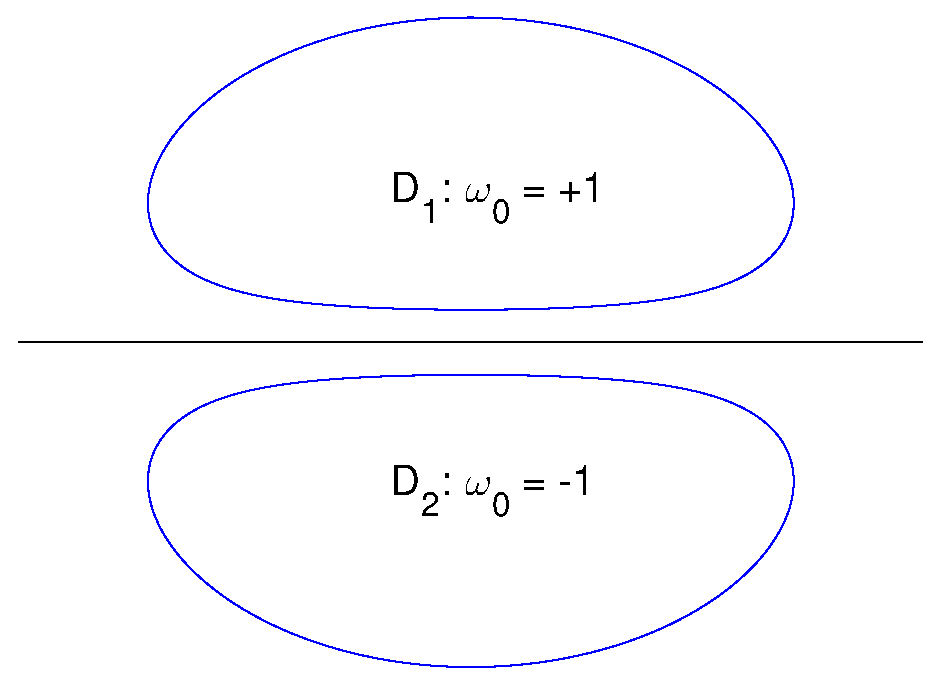
\includegraphics[width=1\linewidth]{pair}
      \caption{A stationary pair of vortex patches.}
    \end{figure}
  \end{minipage}
\end{block}

\begin{alertblock}{Statement of Problem}
  % \begin{alertblock}{Problem}
  For a given choice of length and vorticity $\om$, determine a simple
  differentiable closed curve $\partial D_1$, given by
  $z: [0, 2\pi] \rightarrow \mathbb{C}$, and a corresponding
  translation velocity $U$ so that
  \begin{equation}\label{eq:streamline}
    \im \left[\frac{\dd z}{\dd\nu} \frac{\dd w}{\dd z} \right] = 0
    \quad\text{on $\del D_1$,}
  \end{equation}
  where
  \begin{equation}\label{eq:dw/dz}
    \frac{\dd w}{\dd z}
    = -U + \frac{1}{4\pi} \int_{0}^{2\pi}
    \left(
      \frac{ \conj{z(\nu)-z(\nu')} }{ z(\nu)-z(\nu') }
      + \frac{ \conj{z(\nu)+z(\nu')} }{ z(\nu)+z(\nu') }
    \right)
    z'(\nu') \, \dd \nu'.
    % \frac{dz}{d\nu}(\nu') \,d\nu'.
  \end{equation}
  % \end{alertblock}
\end{alertblock}

% Example: Wingtip vortices
% %%%% Wingtip vortices
% \begin{figure}
%   \includegraphics[width=0.5\linewidth]{wingtip_vortices}
%   \caption{\footnotesize Credit: NASA Langley Research Center, Photo ID:~EL-1996-00130}
% \end{figure}
% %%%%%%%%%%%%%%%%%%%%%%%%%%%%%%%%%%%%%%%%%%%%%%%%%%%%%%%%%%%%%%%%%%%%

\begin{block}{Quasi-solution Method: General Procedures}
  Consider a nonlinear problem written abstractly as $\cN[w] =
  0$:
  \begin{itemize}
  \item Suppose one can find $w_{0}$ which satisfies initial and/or
    boundary conditions within a small error and the residual
    $\cR = \cN[w_{0}]$ is small.
  \item Then the error $E = w - w_0$ must satisfy
    \begin{equation}
      \label{eq:linear}
      \cL[E] = -\cR - \cN_{0}[E] \,,
    \end{equation}
    where $\cL = (\del\cN/\del w)|_{w=w_{0}}$ and
    $\cN_{0}[E] = \cN[w_{0}+E] - \cN[w_{0}] - \cL[E]$.
  \item If $\cL$ has a bounded inverse in some suitable space and
    $\cN_0$ is regular, then $E$ satisfies the weakly nonlinear
    equation
    \begin{equation}
      E = E_0
      - \cL^{-1} \cR - \cL^{-1} \cN_0 [E] \,,
    \end{equation}
    where $E_0$ is a solution to
    % the homogeneous linear problem
    $\cL E = 0$.
  \item The existence and uniqueness of solution to the nonlinear
    fixed point problem can be shown by the \textbf{contraction
      mapping principle}.
  \end{itemize}
\end{block}

\begin{block}{Challenges in Implementing QS Method}
  \begin{itemize}
  \item {\bf Nonlinearity}: the governing
    equation~\eqref{eq:streamline} is nonlinear in
    $z' (\nu)$.
    % since the complex velocity $dW/dz$ also involves $z'(\nu)$.
  \item {\bf Inversion of $\cL$}: need an equivalent formulation in
    which the Fr\'{e}chet derivative of the nonlinear operator at some
    approximate solution has a bounded inverse.
  \item {\bf Choice of solution space}: need to ensure that all
    nonlinear terms are controlled via Banach algebra property.
  \item {\bf Determination of scalar}: it is {\it a priori\/} unclear
    how to analytically determine velocity $U$ for given physical
    configuration.
    % separation of vortex centroids and choice of length and
    % vorticity scales.
  \end{itemize}
\end{block}
%%% Local Variables:
%%% mode: latex
%%% TeX-master: "main"
%%% End:

    \end{column}

    \begin{column}{\sepwid}\end{column}

    \begin{column}{4\tithewid}
      \begin{block}{Conformal Mapping}
  Assuming fore-and-aft symmetry, a conformal map $z=Z (\zeta)$ from the
  conformal domain
  $ \Omega:= \Om^{+} \cup \Om^{-}$
  % $ \Omega:= \left \{ \zeta: \rho < |\zeta| < 1 \right \}$
  to the region
  $\mathcal{D} := \mathcal{D}_{-}\cup\mathcal{D}_{+}$ of the physical
  domain has representation
  \begin{gather}
    \label{eq:conformal}
    Z(\zeta) = \ii a_{0} \left[ \frac{\zeta - \rho}{\zeta + \rho} +
      \alpha(\zeta) - \alpha(\rho^{2}/\zeta) \right]
    \quad\text{with}\quad \alpha(\zeta) = \sum_{k=1}^{\infty} a_{k}
    \zeta^{k} \,,
  \end{gather}
  where $a_{0} \in \RR^{+}$ and $a_{k} \in \RR$ for all $k \in \NN$.

  %%%% Conformal domains %%%%%%%%%%%%%%%%%%%%%%%%%%%%%%%%%%%%%%%%%%%%%%
  \begin{figure}\label{fig:conformal}
    \centering
    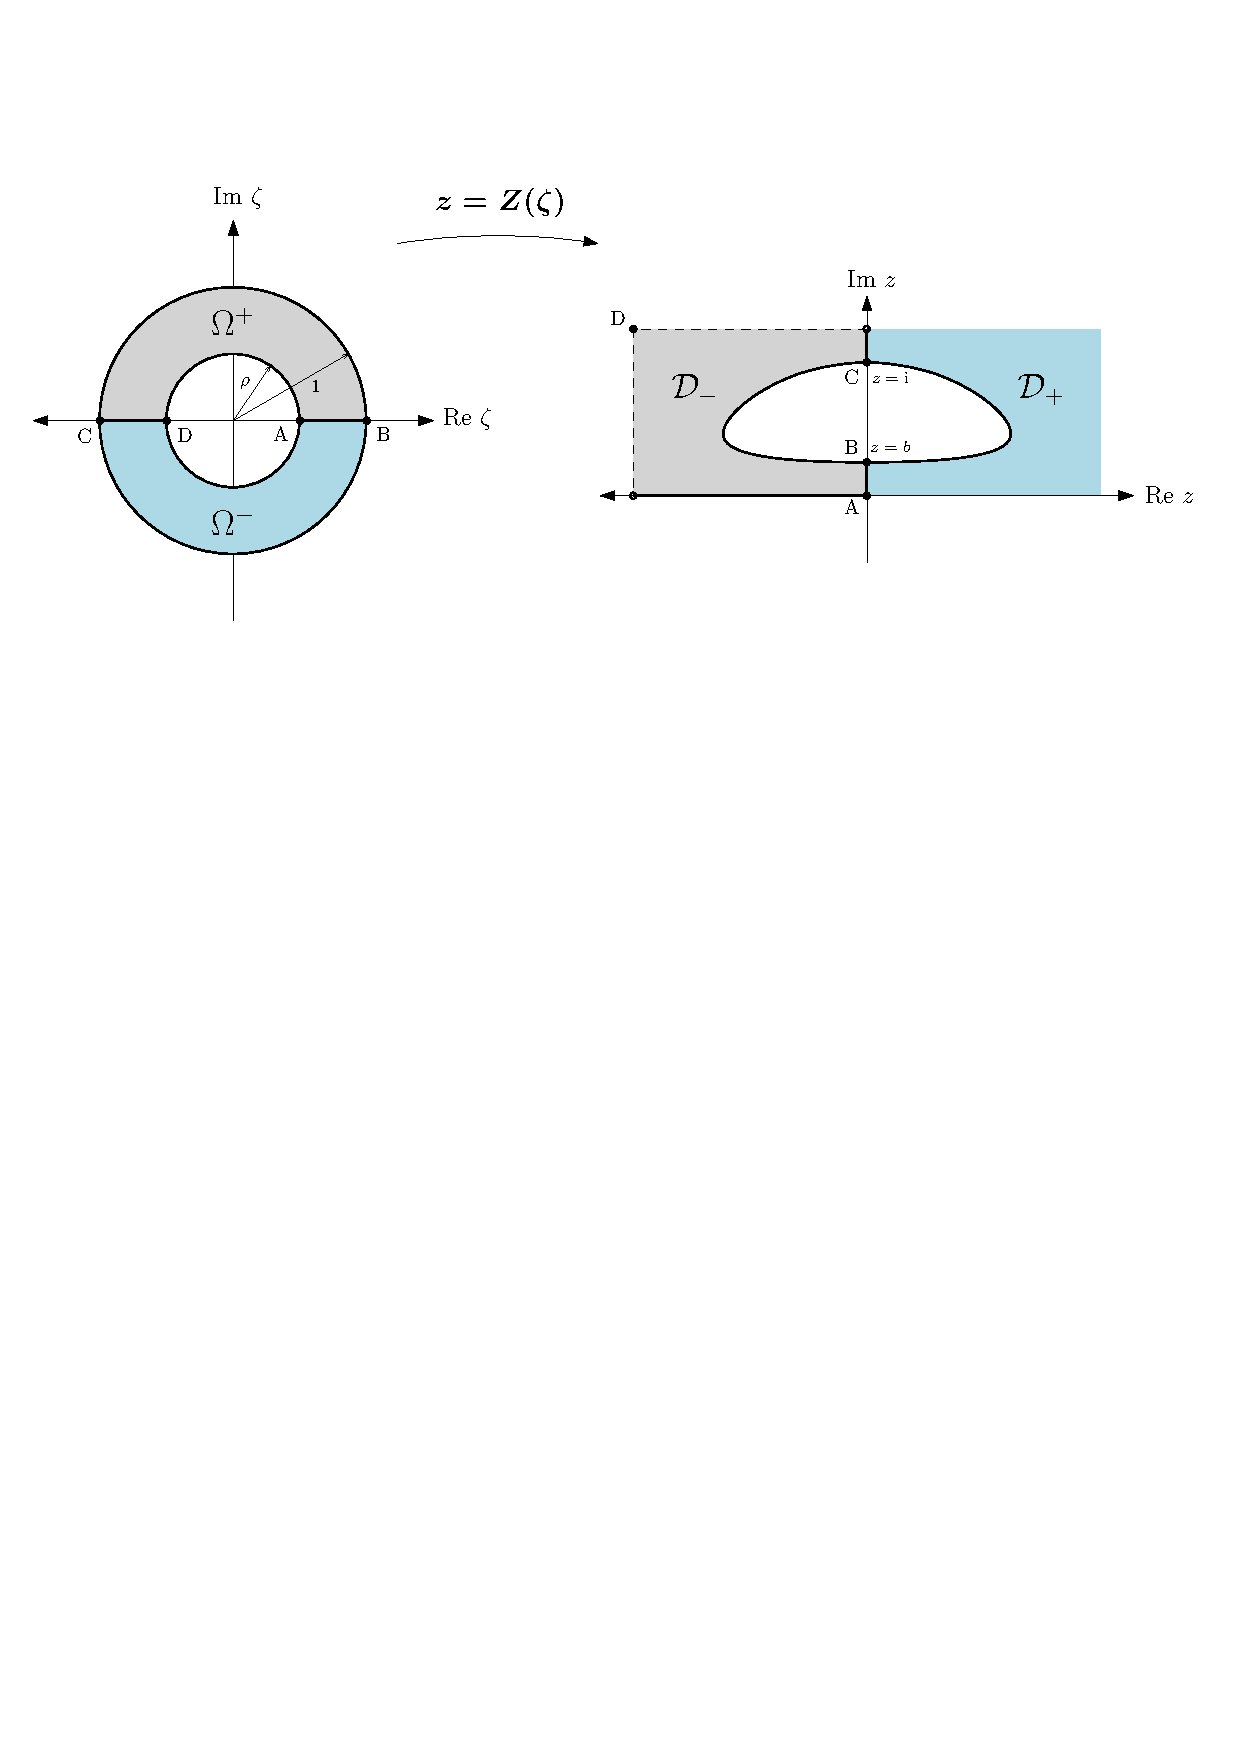
\includegraphics[width=0.95\linewidth]{conformal_continued}
    \caption{Conformal mapping between $\Om$ in the conformal
      $\zeta$-plane and $\cD$ in the physical $z$-plane.}
  \end{figure}

  \textbf{Key observation.}
  \begin{itemize}
  \item $\ii \zeta Z'(\zeta)$ has a double pole at $\zeta = -\rho$
    while $dw/dz - U = O(z^{-2})$ as $z \to \infty$, thus the
    expression
    \begin{equation*}
      \left( \frac{\dd w}{\dd z} - U \right)
      \ii \zeta \frac{\dd Z}{\dd \zeta}
    \end{equation*}
    is singularity-free in $\rho \le \abs{\zeta} \le 1$.
  \item $\ii  \zeta Z'(\zeta) + \cJ(\zeta)$ is singularity-free on
    $\rho \le \abs{\zeta} \le 1$ and is real-valued on
    $\abs{\zeta} = \rho$ and $\abs{\zeta} = 1$ where
    \begin{equation*}
      \mathcal{J} (\zeta) =  2 \zeta \sum_{k=1}^\infty \left[
        \frac{\rho^{2k-1}}{(\zeta+\rho^{2k-1})^2}
        +\frac{\rho^{2k-1}}{(1+\rho^{2k-1} \zeta)^2}
      \right] \,.
    \end{equation*}
  \end{itemize}
\end{block}


\begin{alertblock}{Alternate Formulation: Complex Variable Form}
  Determine a map $Z(\zeta)$ univalent in $\Om$ in the
  form~\eqref{eq:conformal} with $Z'(\zeta)$ existing on $\abs{\zeta}
  = 1$, and a corresponding translation velocity $U$ satisfying
  \begin{equation}\label{eq:complex}
    \Bigl[ U + \cA[Z](\zeta)\Bigr] \ii \zeta Z'(\zeta)
    + U \cJ(\zeta) = \cC[Z] \quad \text{on $\overline{\Om}$,}
  \end{equation}
  where
  \begin{gather}
    \cA[Z](\zeta) = \frac{1}{4\pi} \oint_{\abs{\zeta'}=1}
    \left(
      \frac{ \conj{Z(\zeta) - Z(\zeta')} }
      { Z(\zeta) - Z(\zeta') } +
      \frac{ \conj{Z(\zeta) + Z(\zeta')} }
      { Z(\zeta) + Z(\zeta') }
    \right)
    Z_{\zeta}(\zeta') \; \dd\zeta' \,, \\
    \cC[Z] = \frac{1}{2\pi} \oint_{\abs{\zeta'}=1} \cA[Z](\zeta) Z'(\zeta) \;\dd\zeta \,.
    % \label{eq:J-function}
    % \cJ(\zeta)
    % = 2\zeta \sum_{k=1}^{\infty} \left(
    %   \frac{\rho^{2k-1}}{{\left(\zeta + \rho^{2k-1}\right)}^2}
    %   + \frac{\rho^{2k-1}}{{\left(1 + \rho^{2k-1}\zeta\right)}^2}\
    % \right)\,.
  \end{gather}
\end{alertblock}

\begin{itemize}
\item To deal with highly deformed vortices, \textit{i.e.}, $\rho$ close to 1,
  it is useful to introduce a secondary M\"{o}bius map that maps unit
  circle back to itself:
  \begin{equation}
    \label{eqmobius}
    \zeta = \frac{\eta-\beta}{1-\beta \eta},
    \quad\text{for some suitably choen $\beta \in [0, 1)$.}
  \end{equation}
\item The real coefficients $\left( a_k \right)_{k=1}^\infty $ of the analytic
  function $\alpha$ completely characterize the conformal map $Z$ through the
  representation
  \begin{equation}
    \label{eq1:analytic}
    \alpha \left ( \zeta (\eta) \right ) =
    \sum_{k=1}^\infty a_k \eta^k =
    \sum_{k=1}^\infty a_k \left ( \frac{\zeta+\beta}{1+\beta \zeta} \right )^k
  \end{equation}
  % \item Due to the M\"{o}bius map~\eqref{eqmobius}, the boundary values
  %   of~\eqref{eq:complex} on $\zeta = e^{i\theta}$ can be written in terms of
  %   $\eta = e^{i\nu}$ as follows:
  %   \begin{equation}
  %     \label{eq:1}
  %     z'(\nu) = \theta_{\nu} \frac{C[z] - U j(\nu)}{U + A[z](\nu)}
  %   \end{equation}
  %   where $z(\nu) = Z\left(\zeta(e^{i\nu})\right)$ and $j(\nu) = \cJ\left(\zeta(e^{i\nu})\right)$.
\end{itemize}

%%% Local Variables:
%%% mode: latex
%%% TeX-master: "main"
%%% End:

    \end{column}

    \begin{column}{\sepwid}\end{column}

    \begin{column}{3\tithewid}
      \begin{block}{Main Result}
  \begin{alertblock}{Theorem}
    \label{thm:main}
    For $\rho = \rho_0 \in (0,1)$, there exists a unique solution
    $(U, Z) $ to the vortex patch problem in a small neighborhood of
    $(U_{0}, F_{0})$ where
    \begin{equation}
      \label{eq:41}
      U_{0} = U_0 (\rho)\,, \quad
      F_{0}(\zeta) = i \left[
        \frac{\zeta - \rho}{\zeta + \rho}
        + \alpha(\zeta) - \alpha(\rho^{2}/\zeta) \right] \,.
    \end{equation}
    More precisely,
    \begin{equation}
      \label{eq:thm-error}
      \| Z - F_{0} \| \le 10^{-5} \quad \mbox{and} \quad
      \left| U - U_{0} \right| \le 10^{-5} \,.
    \end{equation}
    Furthermore, this solution $F$ is univalent in the annular domain
    $\Omega$.
  \end{alertblock}

  \begin{itemize}
  \item The expressions for $U_0 $, and analytic function $\alpha$ in the
    unit disk are reported elsewhere~\cite{tk-thesis}.
  \item In principle, a uniform representation of solution for $\rho$ in
    an interval contained in $(0,1)$ can be obtained when the $\rho$
    values contained are modest. When $\rho$ is close to 1, expression
    for accurate quasi-solution is long and hence we refrain from
    presenting uniform formula here.
  \end{itemize}
\end{block}

\begin{block}{Implementation of QS Strategy}
  % We now seek yet another reformulation of the vortex patch problem
  % that is suitable for quasi-solution approach and requires only
  % boundary values on $\abs{\zeta} = 1$.

  \begin{itemize}
  \item Define $(u, G) = (U, Z) - (U_0, F_0)$
    % \begin{equation}
    %   \label{eq:soln-decomp}
    %   (u, G) = (U, Z) - (U_0, F_0) \,.
    % \end{equation}
    where $(U_0, F_0)$ are chosen to make the residual $R_0$ small:
    \begin{equation}
      \label{eq:eqR0}
      R_0 =
      \ii \zeta F_0^\prime (\zeta) - \frac{\cC[F_0] - U_0 \cJ (\zeta) }{ U_0+\cA[F_0] (\zeta) }
      \ .
    \end{equation}
  \item Using the definition of $(u, G)$,~\eqref{eq:complex} may be
    re-written as
    \begin{equation}
      \label{eq:eqG}
      \ii \zeta G_\zeta = -R_0 +
      \frac{\cC[F_0+G] - (U_0 +u) \cJ (\zeta) }{ U_0+u+\cA[F_0 +G] (\zeta) }
      - \frac{\cC[F_0] - U_0 \cJ (\zeta) }{ U_0+\cA[F_0] (\zeta) }
      \ .
    \end{equation}
  \item Since $G$ is completely characterized by its series
    coefficients, it is sufficient to consider the boundary values on
    $\zeta = e^{i\theta}$. Moreover, by the M\"{o}bius map~\eqref{eqmobius},
    the boundary values of~\eqref{eq:eqG} on $\zeta = e^{i\theta}$ can be
    written in terms of the angular variable $\nu$ of $\eta = e^{i\nu}$:
    \begin{equation}
      \label{eq:geq}
      \mathcal{P}_\ge \Bigl (
      g_\nu + \theta_\nu \left [ r_0 - \frac{\cC[f_0+g] - (U_0+u) j)}{U_0+u+ {A}
          [f_0+g]} + \frac{\cC[f_0] - U_0 j }{U_0+ A_0} \right ]
      \Bigr ) = 0 \ ,
    \end{equation}
    where $g (\nu) = G \left ( \zeta (e^{i\nu}) \right )$ and $j(\nu) = \cJ
    \left(  \zeta(e^{i\nu}) \right)$.
  \item The above formulation of the vortex patch problem
    is suitable for quasi-solution approach and requires only
    boundary values on $\abs{\zeta} = 1$.
  \end{itemize}

  % \begin{alertblock}{Alternate Formulation: QS-Method}
  %   Determine $(u, g) \in \RR \times s^2$ such that
  %   \begin{equation}
  %     \label{eq:geq}
  %     \mathcal{P}_\ge \Bigl (
  %     g_\nu + \theta_\nu \left [ r_0 - \frac{\cC[f_0+g] - (U_0+u) j)}{U_0+u+ {A}
  %       [f_0+g]} + \frac{\cC[f_0] - U_0 j }{U_0+ A_0} \right ]
  %     \Bigr ) = 0 \ ,
  %   \end{equation}
  %   and $Z=F_0+G \in \mathcal{F}$, where $g (\nu) = G \left ( \zeta (e^{i\nu}) \right ) $.
  % \end{alertblock}
\end{block}

\begin{block}{References}
  % \nocite{*} % Insert publications even if they are not cited in
  % % the poster
  \small{
    \bibliographystyle{unsrt}   %abbrv, alpha, apalike, plain, siam, unsrt
    \bibliography{tk_ref}
    \vspace{0.75in}
  }
\end{block}


% \setbeamercolor{block title}{fg=red,bg=white} % Change the block title color
% \begin{block}{Acknowledgements}
%   \small{\rmfamily{Nam mollis tristique neque eu
%   luctus. Suspendisse rutrum congue nisi sed
%   convallis. Aenean id neque dolor. Pellentesque habitant
%   morbi tristique senectus et netus et malesuada fames ac
%   turpis egestas.}} \\
% \end{block}

%%% Local Variables:
%%% mode: latex
%%% TeX-master: "main"
%%% End:

    \end{column}

    \begin{column}{\sepwid}\end{column}
  \end{columns}

\end{frame}
\end{document}

%%% Local Variables:
%%% mode: latex
%%% TeX-master: t
%%% End:
